\chapter{Introduction} \label{chap:intro}
Creating a new protocol and ensuring its large scale deployment and use over the internet presents a series of wide ranging challenges. Multipath TCP (MPTCP) has taken many of these considerations into account from the start of its development. For example, it goes to great lengths to ensure retro-compatibility with regular TCP, it has mechanisms for working over Network Address Translators (NATs) and certain other middle boxes, and can use fall-back signaling to revert to TCP if needed. Thanks to this, it has met a level of success which is rare for a protocol of its type. However, there are still many challenges ahead to ensure that the protocol can reach a level of usage comparable to that of regular TCP. \\

One such challenge is security. While securing a protocol itself through the use of randomized  sequence numbers, cryptography, and careful design is important, many attacks use legitimate protocol operations and can only be detected as attacks when looking at the bigger picture. Even when a protocol has been designed to cope with or to mitigate a problem, a network operator may still wish to be alerted when such an attack is taking place. Let's take TCP as an example. If a server receives a SYN packet, replies with a SYN+ACK, and no final ACK arrives, the connection is in a partially opened state until it times out. This is a regular operation and is certainly not a problem from the protocol's point of view. The issue arises when thousands of SYN packets arrive within a short window, a SYN flooding attack. None of the individual connections is odd, but a security system observing the traffic and capable of understanding TCP will easily identify this as an attack. Even with ways to deal with this problem, such as stateless server operation during the connection establishment, the network's operators would likely want to be informed that this attack is happening/has happened. \\

This is just one example to illustrate the need for security and monitoring tools that understand the protocols in use within the network. Many efforts have already been made in order to adapt commonly used tools to MPTCP. For example, Wireshark \cite{wireshark} was patched in order to display MPTCP options and their field values \cite{mpwireshark}, as we can  see in figure \ref{pic:wshark demo}. However, it does not yet provide the function to ``follow'' an MPTCP stream as it can a regular TCP stream. The TCPdump \cite{tcpdump} command line utility was also updated in order to display MPTCP information \cite{mptcpdump}. Both the Wireshark and TCP dump extensions are now featured in the standard distribution of these programs. The packet manipulation program Scapy \cite{scapy} was also given an MPTCP update, allowing it to read, display, modify and write MPTCP options \cite{mpscapy} .   \\

\begin{figure}[!t]
\centering
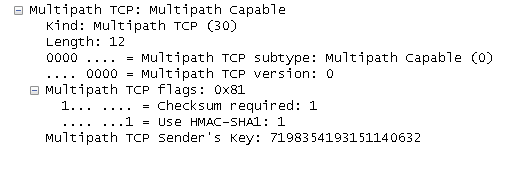
\includegraphics[width=\columnwidth]{Figures/wiresharkdemo.png}
\caption{MPTCP option as seen in Wireshark}
\label{pic:wshark demo}
\end{figure}

This work is intended as a continuation of those efforts in order to bring a new security tool up to speed with MPTCP: Deep Packet Inspection (DPI). DPI is a method generally employed within intrusion detection systems (IDS). While a lot of packet analysis usually stops at headers, DPI can provide byte-level inspection of the whole packet, including the payload. While many systems use DPI, we have chosen to work with the Bro network analysis framework \cite{bro}. Bro is a powerful and flexible system which also has the great advantages of being widely used and open source. As part of our work, we have extended Bro to provide MPTCP comprehension, and built scripts to use these new functionalities for MPTCP analysis. Until now, whenever Bro encountered a packet using MPTCP, it would be treated as a regular TCP packet. Thus, though the operation of the system was not jeopardized, users were incapable of retrieving MPTCP-related information. Furthermore, the subsequent analysis of application-layer protocols became impossible if the MPTCP stream was split over multiple connections, since Bro is incapable of reassembling subflows into a single data stream. \\

This document is split into three main parts. We will begin by presenting the inner workings of the Multipath TCP protocol in chapter \ref{chap:mptcp} and the Bro framework in chapter \ref{chap:bro}. The second part will focus on a first attempt at making the system MPTCP compliant by modifying the TCP Analyzer, for which the source code is available at \url{https://github.com/bbaugnies/DPI-MPTCP}. We will start by describing the modifications to the Bro Engine in chapter \ref{chap:events} . In chapter \ref{chap:script} , we will describe how the modified system can be used to extract meaningful information from analyzed traffic and packet traces through the use of scripts. With the main development explained, chapter \ref{chap:test} will then describe how both the Bro modifications and scripts were tested. Chapter \ref{chap:recap} will serve as a recap for this first implementation, giving a summary of what it can be used for, as well as its shortcomings. The third and final part of this thesis will describe another way to enable Bro to handle MPTCP, specifically aiming at enabling packet reassembly. Chapter \ref{chap:deeper} will first take a deeper look at how TCP reassembly is performed by Bro. Chapter \ref{chap:reassembly} contains a detailed description of the requirements needed to allow this reassembly to work with MPTCP connections. Finally, we will discuss further work which can be done on the subject in chapter \ref{chap:further} .